% =====================================================================
%  Apéndices — Econometría Financiera Aplicada (Jeel Cueva)
% =====================================================================
\appendix

% =====================================================================
\chapter{Herramientas de probabilidad y estadística}\label{ap:prob}
% =====================================================================

Este apéndice reúne los resultados de probabilidad que el libro usa sin demostrar en el texto
principal. Se presentan con la notación de los capítulos: $X,Y$ son variables aleatorias, $\E$ es la
esperanza, $\Var$ la varianza y $\Cov$ la covarianza.

\section{Esperanza, varianza y covarianza}

\begin{proposicion}\label{prop:ap-var}
Para constantes $a,b$ y variables con segundo momento finito,
\[
  \Var(aX+bY)=a^2\Var(X)+b^2\Var(Y)+2ab\Cov(X,Y).
\]
En forma matricial, si $\bm X$ es un vector aleatorio con matriz de covarianzas $\bm\Sigma$ y $\bm w$ un
vector de constantes, $\Var(\bm w'\bm X)=\bm w'\bm\Sigma\bm w$.
\end{proposicion}

\begin{proof}
Sea $\mu_X=\E X$ y $\mu_Y=\E Y$. Por la linealidad de la esperanza:
\begin{align*}
  \Var(aX+bY) &= \E\bigl[(aX+bY-a\mu_X-b\mu_Y)^2\bigr]\\
              &= \E\bigl[(a(X-\mu_X)+b(Y-\mu_Y))^2\bigr]\\
              &= a^2\E\bigl[(X-\mu_X)^2\bigr]+b^2\E\bigl[(Y-\mu_Y)^2\bigr]+2ab\,\E\bigl[(X-\mu_X)(Y-\mu_Y)\bigr]\\
              &= a^2\Var(X)+b^2\Var(Y)+2ab\Cov(X,Y).
\end{align*}
Para la forma matricial, con $\bm\mu=\E\bm X$:
\begin{align*}
  \Var(\bm w'\bm X) &= \E\bigl[(\bm w'\bm X-\bm w'\bm\mu)^2\bigr]\\
                    &= \E\bigl[\bm w'(\bm X-\bm\mu)(\bm X-\bm\mu)'\bm w\bigr]\\
                    &= \bm w'\,\E\bigl[(\bm X-\bm\mu)(\bm X-\bm\mu)'\bigr]\,\bm w\\
                    &= \bm w'\bm\Sigma\bm w. \qedhere
\end{align*}
\end{proof}

La segunda forma es la varianza de un portafolio con pesos $\bm w$ (Capítulos~3 y~12). Como una varianza
no puede ser negativa, $\bm w'\bm\Sigma\bm w\ge0$ para todo $\bm w$: toda matriz de covarianzas es
semidefinida positiva.

\begin{proposicion}[Esperanza iterada]\label{prop:ap-iterada}
Si $\E|X|<\infty$, entonces $\E[X]=\E\bigl[\E(X\mid Y)\bigr]$. En particular, si $\E(u_t\mid
\mathcal F_{t-1})=0$, entonces $\E u_t=0$ y $\Cov(u_t,Z)=0$ para toda $Z$ medible respecto de
$\mathcal F_{t-1}$ con segundo momento finito.
\end{proposicion}

\begin{proof}
La primera parte es la propiedad de la torre de la esperanza condicional. Para la segunda:
\begin{align*}
  \E u_t     &= \E\bigl[\E(u_t\mid\mathcal F_{t-1})\bigr]=\E[0]=0,\\
  \Cov(u_t,Z)&= \E[u_tZ]-\E u_t\,\E Z\\
             &= \E\bigl[\E(u_tZ\mid\mathcal F_{t-1})\bigr]\\
             &= \E\bigl[Z\,\E(u_t\mid\mathcal F_{t-1})\bigr]\\
             &= 0. \qedhere
\end{align*}
\end{proof}

Este resultado justifica que las innovaciones de un modelo GARCH (Capítulo~8) o de un modelo de
expectativas racionales no estén correlacionadas con ninguna información pasada.

\section{Distribuciones derivadas de la normal}

\begin{definicion}
Sean $Z_1,\dots,Z_k$ independientes $N(0,1)$ y $V\sim\chi^2_m$, $W\sim\chi^2_n$ independientes entre sí.
\begin{enumerate}[label=(\roman*)]
  \item $Q=\sum_{i=1}^kZ_i^2$ tiene distribución \emph{chi-cuadrado} con $k$ grados de libertad, $\chi^2_k$.
  \item $t=Z_1/\sqrt{V/m}$, con $Z_1$ independiente de $V$, tiene distribución \emph{$t$ de Student} con $m$
        grados de libertad, $t_m$.
  \item $F=(V/m)/(W/n)$ tiene distribución \emph{$F$ de Snedecor} con $(m,n)$ grados de libertad, $F_{m,n}$.
\end{enumerate}
\end{definicion}

\begin{proposicion}\label{prop:ap-chi}
Si $Q\sim\chi^2_k$, entonces $\E Q=k$ y $\Var Q=2k$.
\end{proposicion}

\begin{proof}
Para $Z\sim N(0,1)$ se cumple $\E Z^2=1$ y $\E Z^4=3$. Entonces:
\begin{align*}
  \E Q          &= \sum_{i=1}^k\E Z_i^2\\
                &= k,\\
  \Var(Z_i^2)   &= \E Z_i^4-(\E Z_i^2)^2\\
                &= 3-1\\
                &= 2,\\
  \Var Q        &= \sum_{i=1}^k\Var(Z_i^2) && \text{(independencia)}\\
                &= 2k. \qedhere
\end{align*}
\end{proof}

Las tres distribuciones se usan en todo el libro: la $\chi^2$ en las pruebas de Wald, de razón de
verosimilitud y de Jarque-Bera; la $t$ en las pruebas sobre un coeficiente y como distribución de las
innovaciones GARCH; la $F$ en las pruebas de restricciones lineales y en la prueba GRS. La
Figura~\ref{fig:apdist} muestra sus densidades. La $t$ tiene colas más pesadas que la normal (con $m=1$
es la distribución de Cauchy, sin media) y converge a la $N(0,1)$ cuando $m\to\infty$; la $\chi^2_k$
es asimétrica a la derecha y se vuelve más simétrica al crecer $k$; y $mF_{m,n}$ converge a $\chi^2_m$
cuando $n\to\infty$.

\begin{figure}[H]
\centering
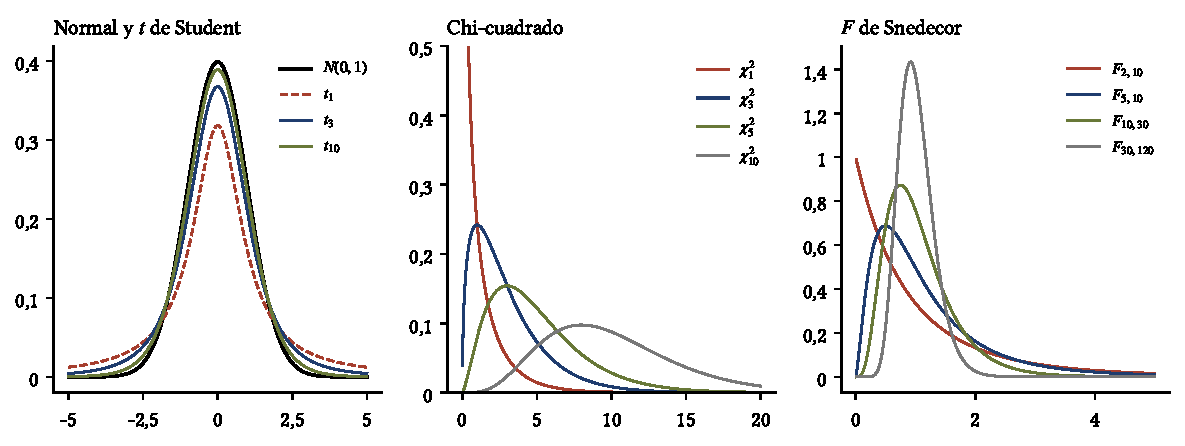
\includegraphics[width=\linewidth]{graficos/apA_fig_distribuciones.pdf}
\caption{Densidades de la normal estándar y de la $t$ de Student (izquierda), de la chi-cuadrado
(centro) y de la $F$ de Snedecor (derecha) para distintos grados de libertad.}
\label{fig:apdist}
\end{figure}

\section{Convergencia y teoremas límite}

\begin{definicion}
Una sucesión $X_T$ \emph{converge en probabilidad} a $c$, $X_T\xrightarrow{p}c$, si para todo
$\varepsilon>0$, $\Pr(|X_T-c|>\varepsilon)\to0$. Converge \emph{en distribución} a $X$,
$X_T\xrightarrow{d}X$, si $\Pr(X_T\le x)\to\Pr(X\le x)$ en todo punto de continuidad de la función de
distribución de $X$.
\end{definicion}

\begin{teorema}[Ley débil de los grandes números]\label{teo:ap-lgn}
Si $X_1,\dots,X_T$ no están correlacionadas, tienen media $\mu$ y varianza $\sigma^2<\infty$, entonces
$\bar X_T\xrightarrow{p}\mu$.
\end{teorema}

\begin{proof}
Por la desigualdad de Chebyshev y la Proposición~\ref{prop:ap-var} (con covarianzas nulas):
\begin{align*}
  \Pr\bigl(|\bar X_T-\mu|>\varepsilon\bigr) &\le \frac{\Var(\bar X_T)}{\varepsilon^2}\\
                                           &= \frac{1}{\varepsilon^2}\cdot\frac{1}{T^2}\sum_{t=1}^T\Var(X_t)\\
                                           &= \frac{\sigma^2}{T\varepsilon^2}\\
                                           &\longrightarrow 0. \qedhere
\end{align*}
\end{proof}

\begin{teorema}[Teorema central del límite de Lindeberg-Lévy]\label{teo:ap-tcl}
Si $X_1,\dots,X_T$ son independientes e idénticamente distribuidas con media $\mu$ y varianza
$\sigma^2\in(0,\infty)$, entonces
\[
  \sqrt T\,\frac{\bar X_T-\mu}{\sigma}\xrightarrow{d}N(0,1).
\]
\end{teorema}

La demostración usa funciones características y puede consultarse en cualquier texto de probabilidad.
Para series temporales existen versiones para diferencias de martingala y para procesos con dependencia
débil (Capítulos~4 y~6), que son las que justifican los errores estándar robustos. La
Figura~\ref{fig:aptcl} ilustra el teorema con una distribución muy asimétrica: la exponencial.

\begin{figure}[H]
\centering
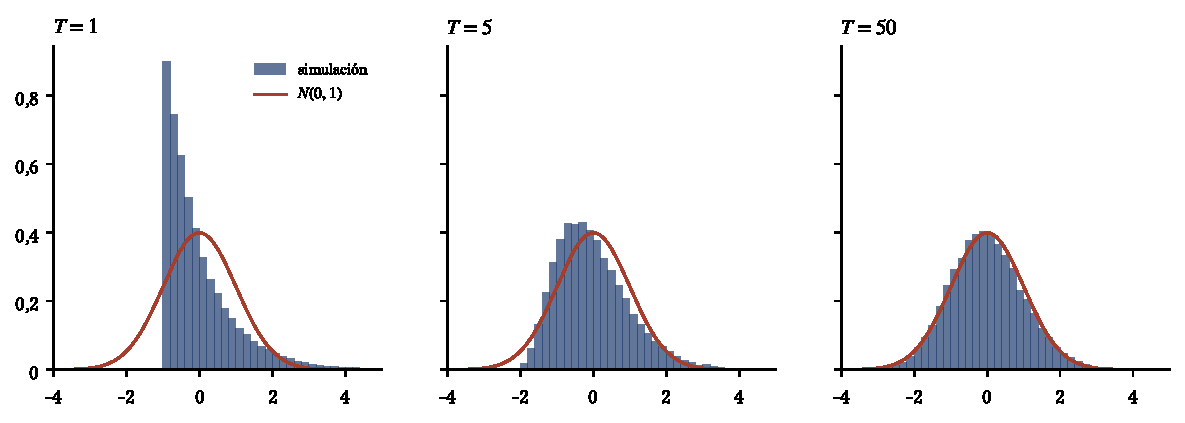
\includegraphics[width=\linewidth]{graficos/apA_fig_tcl.pdf}
\caption{Teorema central del límite: distribución de $\sqrt T(\bar X_T-1)$ con $X_t$ exponenciales de
media y desviación estándar 1, en 50\,000 simulaciones (semilla 2026), para $T=1$, 5 y 50.}
\label{fig:aptcl}
\end{figure}

\begin{teorema}[Slutsky]\label{teo:ap-slutsky}
Si $X_T\xrightarrow{d}X$ y $Y_T\xrightarrow{p}c$, con $c$ constante, entonces $X_T+Y_T\xrightarrow{d}X+c$,
$X_TY_T\xrightarrow{d}cX$ y, si $c\ne0$, $X_T/Y_T\xrightarrow{d}X/c$.
\end{teorema}

Por el teorema de Slutsky, se puede reemplazar $\sigma$ por un estimador consistente $\hat\sigma$ en el
TCL sin cambiar la distribución límite: así se obtienen los estadísticos $t$ asintóticos.

\begin{teorema}[Método delta]\label{teo:ap-delta}
Si $\sqrt T(\hat{\bm\theta}-\bm\theta)\xrightarrow{d}N(\bm0,\bm V)$ y $g$ es una función con gradiente
$\nabla g(\bm\theta)\ne\bm0$ continuo en $\bm\theta$, entonces
\[
  \sqrt T\bigl(g(\hat{\bm\theta})-g(\bm\theta)\bigr)\xrightarrow{d}
  N\bigl(0,\ \nabla g(\bm\theta)'\,\bm V\,\nabla g(\bm\theta)\bigr).
\]
\end{teorema}

\begin{proof}[Idea de la demostración]
Por el teorema del valor medio, existe $\bar{\bm\theta}$ entre $\hat{\bm\theta}$ y $\bm\theta$ tal que
\begin{align*}
  g(\hat{\bm\theta})                     &= g(\bm\theta)+\nabla g(\bar{\bm\theta})'(\hat{\bm\theta}-\bm\theta),\\
  \sqrt T\bigl(g(\hat{\bm\theta})-g(\bm\theta)\bigr) &= \nabla g(\bar{\bm\theta})'\,\sqrt T(\hat{\bm\theta}-\bm\theta).
\end{align*}
Como $\hat{\bm\theta}\xrightarrow{p}\bm\theta$, también $\bar{\bm\theta}\xrightarrow{p}\bm\theta$ y, por la
continuidad del gradiente, $\nabla g(\bar{\bm\theta})\xrightarrow{p}\nabla g(\bm\theta)$. Por el teorema de
Slutsky, el lado derecho converge a $\nabla g(\bm\theta)'\bm Y$ con $\bm Y\sim N(\bm0,\bm V)$, cuya
varianza es $\nabla g(\bm\theta)'\bm V\nabla g(\bm\theta)$ (Proposición~\ref{prop:ap-var}).
\end{proof}

\section{Ejercicio resuelto}

\begin{ejresuelto}{Precisión de la razón media/desviación de \texttt{EPU} y del S\&P 500}\label{ej:apdelta}
\enunciado Sea $\theta=\mu/\sigma$ la razón entre la media y la desviación estándar del rendimiento
mensual (la razón de Sharpe cuando la tasa libre de riesgo es cero). (a) Con el método delta, obtenga la
varianza asintótica de $\hat\theta=\hat\mu/\hat\sigma$ para rendimientos independientes con asimetría
$\gamma_3$ y curtosis $\gamma_4$, y su caso normal. (b) Calcule $\hat\theta$, su error estándar y un
intervalo de confianza del 95\,\% para \texttt{EPU} y el S\&P 500, con datos mensuales de 2015--2025.

\solucion
\paso{Paso 1. Distribución conjunta de $(\hat\mu,\hat\sigma^2)$.} Con $\mu_j=\E(R-\mu)^j$, se cumple
\begin{align*}
  \Var(\hat\mu)          &\approx \frac{\sigma^2}{T},\\
  \Cov(\hat\mu,\hat\sigma^2) &\approx \frac{\mu_3}{T},\\
  \Var(\hat\sigma^2)     &\approx \frac{\mu_4-\sigma^4}{T}.
\end{align*}
\paso{Paso 2. Gradiente.} Con $g(a,b)=a/\sqrt b$, evaluado en $(\mu,\sigma^2)$:
\begin{align*}
  \frac{\partial g}{\partial a} &= \frac{1}{\sqrt b}=\frac1\sigma,\\
  \frac{\partial g}{\partial b} &= -\frac{a}{2b^{3/2}}=-\frac{\mu}{2\sigma^3}.
\end{align*}
\paso{Paso 3. Método delta.} Por el Teorema~\ref{teo:ap-delta}, $T\Var(\hat\theta)\approx v$ con
\begin{align*}
  v &= \frac{1}{\sigma^2}\sigma^2+2\cdot\frac1\sigma\cdot\Bigl(-\frac{\mu}{2\sigma^3}\Bigr)\mu_3
       +\frac{\mu^2}{4\sigma^6}\bigl(\mu_4-\sigma^4\bigr)\\
    &= 1-\frac{\mu}{\sigma}\cdot\frac{\mu_3}{\sigma^3}+\frac{\mu^2}{4\sigma^2}\Bigl(\frac{\mu_4}{\sigma^4}-1\Bigr)\\
    &= 1-\theta\gamma_3+\frac{\theta^2}{4}(\gamma_4-1).
\end{align*}
Bajo normalidad, $\gamma_3=0$ y $\gamma_4=3$, de modo que
\begin{align*}
  v &= 1+\frac{\theta^2}{4}(3-1)\\
    &= 1+\frac{\theta^2}{2}.
\end{align*}
\paso{Paso 4. Cálculo.}

\codigoweb{apA_ej01}
\salidaR{apA_ej01_R.txt}
\lectura{apA_ej01}

\RvsPy Ambos programas calculan los momentos con divisor $T$, tal como aparecen en el Paso~1, y dan
las mismas cifras.

\begin{conclusion}
Con 132 meses, el error estándar de $\hat\theta$ es cercano a $1/\sqrt{132}\approx0{,}087$ en ambas
series. Esa precisión es baja: el intervalo del 95\,\% para \texttt{EPU} incluye el cero, así que once años
de datos no bastan para afirmar que su rendimiento medio fue positivo. El del S\&P 500 lo excluye por
poco. La corrección por asimetría negativa y curtosis aumenta el error estándar entre 2\,\% y 5\,\%.
\end{conclusion}
\end{ejresuelto}

\section{Ejercicios propuestos}

\begin{enumerate}[label=\textbf{A.\arabic*},leftmargin=*,itemsep=6pt]
  \item Demuestre que si $X\sim N(\mu,\sigma^2)$, entonces $\E e^{X}=e^{\mu+\sigma^2/2}$, y úselo para
        obtener la media de un precio lognormal (Capítulo~1).
  \item Demuestre que si $t\sim t_m$ con $m>2$, entonces $\Var(t)=m/(m-2)$, y explique por qué el
        Capítulo~8 reescala las innovaciones $t$ para que tengan varianza unitaria.
  \item Use el método delta para obtener el error estándar de la volatilidad anualizada
        $\hat\sigma\sqrt{252}$ a partir de $\Var(\hat\sigma^2)\approx(\mu_4-\sigma^4)/T$. Aplíquelo a los
        rendimientos diarios de \texttt{BVN} del Ejercicio~\ref{ej:anualizar}.
  \item \emph{(Simulación.)} Repita la Figura~\ref{fig:aptcl} con rendimientos $t_3$ en lugar de
        exponenciales. ¿Converge más rápido o más lento? ¿Y con $t_2$, que no tiene varianza finita?
\end{enumerate}

% =====================================================================
\chapter{Álgebra matricial para econometría}\label{ap:matrices}
% =====================================================================

\section{Definiciones básicas}

Una matriz cuadrada $\bm A$ es \emph{simétrica} si $\bm A=\bm A'$, \emph{idempotente} si $\bm A\bm A=\bm A$
y \emph{definida positiva} si $\bm x'\bm A\bm x>0$ para todo $\bm x\ne\bm0$ (semidefinida positiva si
$\ge0$). La \emph{traza} es la suma de la diagonal, $\operatorname{tr}\bm A=\sum_ia_{ii}$, y cumple
$\operatorname{tr}(\bm A\bm B)=\operatorname{tr}(\bm B\bm A)$ siempre que ambos productos existan. El
\emph{rango} de $\bm X$ ($T\times k$) es el número de columnas linealmente independientes; si
$\operatorname{rango}\bm X=k$, la matriz $\bm X'\bm X$ es definida positiva y, por tanto, invertible.

\begin{proposicion}\label{prop:ap-xx}
Si $\operatorname{rango}\bm X=k$, entonces $\bm X'\bm X$ es definida positiva.
\end{proposicion}

\begin{proof}
Sea $\bm c\ne\bm0$ y $\bm v=\bm X\bm c$. Como las columnas de $\bm X$ son linealmente independientes,
$\bm v\ne\bm0$. Entonces
\begin{align*}
  \bm c'\bm X'\bm X\bm c &= (\bm X\bm c)'(\bm X\bm c)\\
                         &= \bm v'\bm v\\
                         &= \sum_{t=1}^Tv_t^2\\
                         &> 0. \qedhere
\end{align*}
\end{proof}

\section{Derivadas de formas lineales y cuadráticas}

\begin{proposicion}\label{prop:ap-deriv}
Sean $\bm a$ y $\bm x$ vectores $k\times1$ y $\bm A$ una matriz $k\times k$. Entonces
\[
  \frac{\partial\,\bm a'\bm x}{\partial\bm x}=\bm a,\qquad
  \frac{\partial\,\bm x'\bm A\bm x}{\partial\bm x}=(\bm A+\bm A')\bm x,
\]
que es igual a $2\bm A\bm x$ cuando $\bm A$ es simétrica.
\end{proposicion}

\begin{proof}
Para la forma lineal, $\bm a'\bm x=\sum_ia_ix_i$, y su derivada respecto de $x_j$ es $a_j$. Para la
forma cuadrática:
\begin{align*}
  \bm x'\bm A\bm x &= \sum_{i=1}^k\sum_{l=1}^k a_{il}x_ix_l,\\
  \frac{\partial\,\bm x'\bm A\bm x}{\partial x_j} &= \sum_{l=1}^ka_{jl}x_l+\sum_{i=1}^ka_{ij}x_i\\
                                                   &= (\bm A\bm x)_j+(\bm A'\bm x)_j .
\end{align*}
Apilando las $k$ derivadas se obtiene $(\bm A+\bm A')\bm x$.
\end{proof}

\section{Mínimos cuadrados en forma matricial}

\begin{proposicion}\label{prop:ap-mco}
Sea $\bm y=\bm X\bm\beta+\bm u$, con $\bm X$ de rango $k$. El vector que minimiza
$S(\bm b)=(\bm y-\bm X\bm b)'(\bm y-\bm X\bm b)$ es $\hat{\bm\beta}=(\bm X'\bm X)^{-1}\bm X'\bm y$.
\end{proposicion}

\begin{proof}
Expandimos la suma de cuadrados y derivamos con la Proposición~\ref{prop:ap-deriv}:
\begin{align*}
  S(\bm b) &= \bm y'\bm y-\bm b'\bm X'\bm y-\bm y'\bm X\bm b+\bm b'\bm X'\bm X\bm b\\
           &= \bm y'\bm y-2\bm y'\bm X\bm b+\bm b'\bm X'\bm X\bm b,\\
  \frac{\partial S}{\partial\bm b} &= -2\bm X'\bm y+2\bm X'\bm X\bm b .
\end{align*}
Igualando a cero se obtienen las ecuaciones normales:
\begin{align*}
  \bm X'\bm X\hat{\bm\beta} &= \bm X'\bm y,\\
  \hat{\bm\beta}            &= (\bm X'\bm X)^{-1}\bm X'\bm y .
\end{align*}
La matriz de segundas derivadas es $2\bm X'\bm X$, definida positiva por la
Proposición~\ref{prop:ap-xx}, así que el punto crítico es el mínimo global.
\end{proof}

\begin{proposicion}[Matrices de proyección]\label{prop:ap-proy}
Sean $\bm P=\bm X(\bm X'\bm X)^{-1}\bm X'$ y $\bm M=\bm I-\bm P$. Entonces $\bm P$ y $\bm M$ son
simétricas e idempotentes, $\bm P\bm X=\bm X$, $\bm M\bm X=\bm0$, los valores ajustados son
$\hat{\bm y}=\bm P\bm y$, los residuos son $\hat{\bm u}=\bm M\bm y=\bm M\bm u$ y
$\operatorname{tr}\bm M=T-k$.
\end{proposicion}

\begin{proof}
La simetría es inmediata porque $(\bm X'\bm X)^{-1}$ es simétrica. Idempotencia y anulación:
\begin{align*}
  \bm P\bm P &= \bm X(\bm X'\bm X)^{-1}\bm X'\bm X(\bm X'\bm X)^{-1}\bm X'\\
             &= \bm X(\bm X'\bm X)^{-1}\bm X'\\
             &= \bm P,\\
  \bm P\bm X &= \bm X(\bm X'\bm X)^{-1}\bm X'\bm X\\
             &= \bm X,\\
  \bm M\bm X &= \bm X-\bm P\bm X\\
             &= \bm 0,\\
  \bm M\bm M &= \bm I-2\bm P+\bm P\bm P\\
             &= \bm M .
\end{align*}
Los residuos y la traza:
\begin{align*}
  \hat{\bm u} &= \bm y-\bm X\hat{\bm\beta}\\
              &= \bm y-\bm P\bm y\\
              &= \bm M\bm y\\
              &= \bm M(\bm X\bm\beta+\bm u)\\
              &= \bm M\bm u,\\
  \operatorname{tr}\bm P &= \operatorname{tr}\bigl((\bm X'\bm X)^{-1}\bm X'\bm X\bigr)\\
                         &= \operatorname{tr}\bm I_k\\
                         &= k,\\
  \operatorname{tr}\bm M &= T-k. \qedhere
\end{align*}
\end{proof}

La traza de $\bm M$ explica el divisor $T-k$ del estimador insesgado de la varianza del error: como
$\E(\hat{\bm u}'\hat{\bm u})=\E(\bm u'\bm M\bm u)=\sigma^2\operatorname{tr}\bm M=\sigma^2(T-k)$ cuando
$\E(\bm u\bm u'\mid\bm X)=\sigma^2\bm I$.

\section{El teorema de Frisch-Waugh-Lovell}

\begin{teorema}[Frisch-Waugh-Lovell]\label{teo:ap-fwl}
Particione $\bm X=[\bm X_1\ \bm X_2]$ y $\hat{\bm\beta}=(\hat{\bm\beta}_1',\hat{\bm\beta}_2')'$, y sea
$\bm M_1=\bm I-\bm X_1(\bm X_1'\bm X_1)^{-1}\bm X_1'$. Entonces
\[
  \hat{\bm\beta}_2=(\bm X_2'\bm M_1\bm X_2)^{-1}\bm X_2'\bm M_1\bm y,
\]
es decir, $\hat{\bm\beta}_2$ se obtiene regresando los residuos de $\bm y$ sobre $\bm X_1$ en los
residuos de $\bm X_2$ sobre $\bm X_1$.
\end{teorema}

\begin{proof}
Escribimos $\bm y=\bm X_1\hat{\bm\beta}_1+\bm X_2\hat{\bm\beta}_2+\hat{\bm u}$, donde $\hat{\bm u}$ es
ortogonal a $\bm X_1$ y a $\bm X_2$ por las ecuaciones normales. Premultiplicamos por $\bm M_1$, que anula
a $\bm X_1$ y deja intacto a $\hat{\bm u}$ (porque $\bm X_1'\hat{\bm u}=\bm0$):
\begin{align*}
  \bm M_1\bm y &= \bm M_1\bm X_1\hat{\bm\beta}_1+\bm M_1\bm X_2\hat{\bm\beta}_2+\bm M_1\hat{\bm u}\\
               &= \bm M_1\bm X_2\hat{\bm\beta}_2+\hat{\bm u}.
\end{align*}
Premultiplicamos por $\bm X_2'$ y usamos $\bm X_2'\hat{\bm u}=\bm0$:
\begin{align*}
  \bm X_2'\bm M_1\bm y &= \bm X_2'\bm M_1\bm X_2\hat{\bm\beta}_2+\bm X_2'\hat{\bm u}\\
                       &= \bm X_2'\bm M_1\bm X_2\hat{\bm\beta}_2,\\
  \hat{\bm\beta}_2     &= (\bm X_2'\bm M_1\bm X_2)^{-1}\bm X_2'\bm M_1\bm y . \qedhere
\end{align*}
\end{proof}

El teorema explica por qué incluir una constante equivale a trabajar con datos centrados, por qué los
efectos fijos del Capítulo~19 se estiman con datos en desviaciones respecto de la media de cada
individuo, y por qué el coeficiente de un factor en una regresión múltiple (Capítulo~14) mide su efecto
\emph{neto} de los demás factores.

\section{Producto de Kronecker y operador vec}

El producto de Kronecker de $\bm A$ ($m\times n$) y $\bm B$ ($p\times q$) es la matriz $mp\times nq$
\[
  \bm A\otimes\bm B=\begin{pmatrix}a_{11}\bm B&\cdots&a_{1n}\bm B\\ \vdots&\ddots&\vdots\\
                    a_{m1}\bm B&\cdots&a_{mn}\bm B\end{pmatrix},
\]
y $\operatorname{vec}\bm A$ apila las columnas de $\bm A$ en un vector $mn\times1$. Se usan para escribir
los modelos VAR (Capítulo~10) y los sistemas de ecuaciones de forma compacta.

\begin{proposicion}\label{prop:ap-vec}
Para matrices conformables, $\operatorname{vec}(\bm A\bm B\bm C)=(\bm C'\otimes\bm A)\operatorname{vec}\bm B$.
\end{proposicion}

\begin{proof}
Sea $\bm b_l$ la columna $l$ de $\bm B$ y $c_{lj}$ el elemento $(l,j)$ de $\bm C$. La columna $j$ de
$\bm A\bm B\bm C$ es
\begin{align*}
  (\bm A\bm B\bm C)_{\cdot j} &= \bm A\,(\bm B\bm C)_{\cdot j}\\
                              &= \bm A\sum_lc_{lj}\bm b_l\\
                              &= \sum_l c_{lj}\,\bm A\bm b_l\\
                              &= \bigl(c_{1j}\bm A\ \ c_{2j}\bm A\ \cdots\bigr)\operatorname{vec}\bm B .
\end{align*}
El bloque $(c_{1j}\bm A\ \ c_{2j}\bm A\ \cdots)$ es la fila de bloques $j$ de $\bm C'\otimes\bm A$, porque
el elemento $(j,l)$ de $\bm C'$ es $c_{lj}$. Apilando las columnas $j=1,2,\dots$ se obtiene el resultado.
\end{proof}

\section{Ejercicios propuestos}

\begin{enumerate}[label=\textbf{B.\arabic*},leftmargin=*,itemsep=6pt]
  \item Demuestre que $\operatorname{tr}(\bm A\bm B)=\operatorname{tr}(\bm B\bm A)$ y úselo para probar
        que $\E(\bm u'\bm M\bm u)=\sigma^2(T-k)$.
  \item Verifique numéricamente el Teorema~\ref{teo:ap-fwl} con los datos del Ejercicio~\ref{ej:portafolio}:
        regrese el rendimiento mensual de \texttt{BAP} sobre una constante, \texttt{SCCO} y \texttt{BVN},
        y compare el coeficiente de \texttt{BVN} con el de la regresión de residuos.
  \item Demuestre que los valores propios de una matriz idempotente son 0 o 1 y que su rango es igual a
        su traza.
  \item Demuestre que $(\bm A\otimes\bm B)(\bm C\otimes\bm D)=\bm A\bm C\otimes\bm B\bm D$ y que
        $(\bm A\otimes\bm B)^{-1}=\bm A^{-1}\otimes\bm B^{-1}$ cuando las inversas existen.
\end{enumerate}

% =====================================================================
\chapter{Datos, programas y reproducibilidad}\label{ap:datos}
% =====================================================================

\section{Organización del proyecto}

Todos los resultados numéricos del libro son la salida real de un programa. El proyecto se organiza
así:
\begin{itemize}[leftmargin=*]
  \item \texttt{capitulos/}: un archivo \texttt{.tex} por capítulo; \texttt{main.tex} los reúne.
  \item \texttt{datos/peru/} y \texttt{datos/internacional/}: series descargadas, en CSV, con un archivo
        \texttt{FUENTES.txt} que documenta el origen y la fecha de descarga de cada una.
  \item \texttt{codigo/R/} y \texttt{codigo/Python/}: un programa por ejercicio
        (\texttt{capNN\_ejMM.R} y \texttt{capNN\_ejMM.py}). Para que el libro no se haga extenso, los programas
        no se imprimen: están completos, con sus salidas en ambos lenguajes, en el repositorio del libro en GitHub (véase el Prefacio).
  \item \texttt{salidas/}: la salida de consola de cada programa; el libro inserta tal cual la salida en R.
  \item \texttt{graficos/}: figuras en PDF generadas por los programas de Python.
  \item \texttt{lecturas/}: las tablas ``Cómo leer la salida'' que siguen a cada salida de R. Su texto está
        en la subcarpeta \texttt{fuente/} y el programa \texttt{generar.py} las convierte en tablas.
\end{itemize}
Los programas se ejecutan desde la carpeta raíz del proyecto:
\begin{lstlisting}[style=salida,title={\small\sffamily\color{gray}Terminal}]
Rscript codigo/R/cap01_ej01.R > salidas/cap01_ej01_R.txt
PYTHONPATH=codigo/Python python3 codigo/Python/cap01_ej01.py > salidas/cap01_ej01_Py.txt
\end{lstlisting}
Se requiere R base (y el paquete \texttt{jsonlite} solo para descargar datos) y, en Python, \texttt{numpy},
\texttt{pandas}, \texttt{scipy}, \texttt{statsmodels} y \texttt{matplotlib}; \texttt{arch} y
\texttt{linearmodels} se usan para comprobar los cálculos programados a mano.

\section{Descarga de los datos peruanos}

Las series del BCRP se obtienen de la API pública de BCRPData, cuya dirección tiene la forma
\begin{center}\small
\texttt{https://estadisticas.bcrp.gob.pe/estadisticas/series/api/}\textit{código}\texttt{/json/}\textit{inicio}\texttt{/}\textit{fin}
\end{center}
con fechas diarias escritas sin ceros a la izquierda (por ejemplo, \texttt{2015-1-2}). La respuesta trae
cada dato como texto, con la fecha en la forma \texttt{31.Dic.14} y el valor \texttt{n.d.} cuando no hay
dato. Las acciones se obtienen del punto de acceso \texttt{v8/finance/chart} de Yahoo Finance, que
devuelve el cierre, el cierre ajustado, los dividendos y los desdoblamientos. Este punto de acceso no es
una API oficial y puede cambiar sin aviso; los paquetes \texttt{quantmod} (R) y \texttt{yfinance} (Python)
ofrecen alternativas.

Los programas \texttt{apC\_descarga.R} y \texttt{apC\_descarga.py}, publicados en el repositorio del libro,
reproducen la descarga. \emph{No se ejecutan al compilar el libro} porque requieren conexión a internet;
los archivos de \texttt{datos/peru/} se obtuvieron con estas mismas consultas el 8 y el 9 de noviembre de
2026 y se verificaron dato por dato con sumas de control.

\codigoweb{apC_descarga}

\section{Inventario de los datos peruanos}

El programa \texttt{apC\_inventario.R} recorre \texttt{datos/peru/} y muestra el número de filas, la primera y la última
fecha y el valor correspondiente de cada archivo. Es la verificación que respalda la
Tabla~\ref{tab:fuentes1}.

\codigoweb{apC_inventario}
\salidaR{apC_inventario_R.txt}
\lectura{apC_inventario}

\RvsPy R lee los archivos como texto (\texttt{colClasses = "character"}), por lo que muestra los
valores exactamente como están guardados; pandas los convierte en números y elimina los ceros finales
(por ejemplo, \texttt{2.99300} se muestra como \texttt{2.993}).

\section{Problemas encontrados en los datos y cómo se resolvieron}

\begin{table}[H]
\centering\small
\begin{tabularx}{\linewidth}{@{}lXX@{}}
\toprule
Serie & Problema & Tratamiento \\
\midrule
BVL (BCRP) & 21-jun-2024: 22\,521,03 entre 29\,857,57 y 30\,058,66 & Se elimina el dato (Ejercicios~\ref{ej:logsimple} y~\ref{ej:anualizar}) \\
BVL (BCRP) & Hasta 2020 repite el valor en feriados peruanos & Se conserva; se advierte al contar días por año \\
BCRP & Desde 2021, feriados como \texttt{n.d.} & Se omiten esas fechas \\
\texttt{BAP} (Yahoo) & Dividendo de abril de 2020 registrado dos veces & Se corrige el precio ajustado (Ejercicio~\ref{ej:dividendos}) \\
\texttt{SCCO} (Yahoo) & Dividendos en acciones de 2024--2026 tratados como desdoblamientos & El cierre ya viene ajustado; se usa el cierre ajustado \\
\texttt{PEN=X} (Yahoo) & Difiere del tipo de cambio oficial hasta en 2,7 puntos por año & Se prefiere el BCRP (Ejercicio~\ref{ej:soles}) \\
\texttt{\^{}SPBLPGPT} & Yahoo ya no devuelve datos & Se usa la serie \texttt{PD38026MD} del BCRP \\
\bottomrule
\end{tabularx}
\caption{Problemas detectados en los datos del Capítulo 1 y su tratamiento.}
\label{tab:problemasdatos}
\end{table}

\section{Recomendaciones de trabajo}

\begin{enumerate}[leftmargin=*]
  \item Guarde siempre una copia de los datos tal como se descargaron y registre la fecha de descarga: los
        precios ajustados cambian con cada nuevo dividendo (Proposición~\ref{prop:ajuste}).
  \item Nunca corrija un dato a mano dentro del archivo original. Escriba la corrección en el programa,
        con un comentario, para que cualquiera pueda ver y revertir la decisión.
  \item Antes de modelar, mire los rendimientos más extremos y compruebe si son errores, eventos
        corporativos o información genuina.
  \item Fije la semilla de toda simulación (en este libro, \texttt{2026} salvo indicación) para que los
        resultados se puedan reproducir.
  \item Compare siempre R y Python: si dos implementaciones independientes dan la misma cifra, es poco
        probable que ambas tengan el mismo error.
\end{enumerate}
